\chapter{Indledning}
\chapter{Kravspecifikation}
\section{Godkendelsesformular}
\begin{table}[h!]
\label{tab:tabel2}
\begin{tabular}{| l | >{\raggedright\arraybackslash}p{12cm} |}
   \hline
   \textbf{Forfattere} & Line, Mette, Brian, Mohamed, Khaled og Ida\\ \hline
   \textbf{Godkendes af:} & Samuel Alberg Thrysøe\\ \hline
   \textbf{Antal sider:} & \\ \hline
   \textbf{Kunde:} & IHA\\ \hline
\end{tabular}
\end{table}
\textbf{Ved underskrivelse af dette dokument accepteres det af begge parter, som værende kravene til udviklingen af det ønskede system.}
\newline
\textbf{Sted og dato:}\\
\\
\\
\begin{table}
[h!]
\begin{tabular}{ l lllllllll l}
--------------------------------------&&&&&&&&&&--------------------------------------\\ 
Kundens underskrift &&&&&&&&&&Leverandørens underskrift\\
\end{tabular}
\end{table}
\section{Indledning}
Denne kravsspecifikation er blevet uadarbejdet åå baggrund af krav fra kunden, samt hvad leverandøren finder muligt. Kravsspecifikationens formål er at specificere de krav de er til produktet.
\newpage

\section{Systembeskrivelse}

\newpage

\section{Aktør-kontekst diagram}
\begin{figure}[h!]
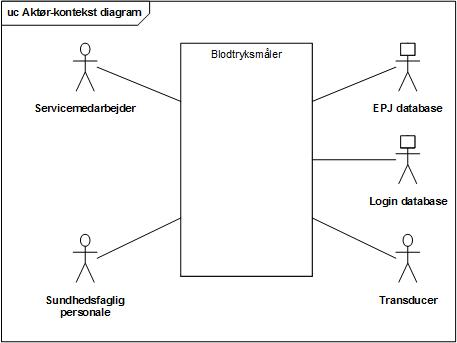
\includegraphics[width =0.65\textwidth , left]{billeder/Aktorkontekst.jpg}
\caption{\textbf{Aktør-kontekst diagram}}
\end{figure}

Af dette diagram ses de interagerende aktører: \textit{Sundhedsfaglig personale}, \textit{Transducer}, \textit{EPJ database}, \textit{Login database} og \textit{Servicemedarbejder}.\\ Herunder er der en detaljeret beskrivelse af hver aktør.

\begin{table}[h!]
\begin{tabular}{| >{\raggedright\arraybackslash}p{3cm} | >{\raggedright\arraybackslash}p{12cm} |}
   \hline
   Navn: & Sundhedsfaglig personale\\ \hline
   Type: & Primær aktør \\ \hline
   Beskrivelse: & Det sundhedsfaglige personale er aktøren der påsætter måleudstyret på transduceren, samt starter målingen. Det er det sundhedsfaglige personale, der interagerer med systemet og dermed har tilgang til de viste målinger på brugergrænse skærmene (startskærm og hovedskærm).\\ \hline
\end{tabular}
\end{table}


\begin{table}[h!]
\begin{tabular}{| >{\raggedright\arraybackslash}p{3cm} | >{\raggedright\arraybackslash}p{12cm} |}
   \hline
   Navn: & Transducer\\ \hline
   Type: & Sekundær aktør \\ \hline
   Beskrivelse: & Transduceren er kilden til måleresultaterne, og dermed fungerer som patienten. Måleresultater opnås ved, at disse data sendes ind i systemet igennem hardwaren.\\ \hline
\end{tabular}
\end{table}


\begin{table}[h!]
\begin{tabular}{| >{\raggedright\arraybackslash}p{3cm} | >{\raggedright\arraybackslash}p{12cm} |}
   \hline
   Navn: & Login database\\ \hline
   Type: & Sekundær aktør \\ \hline
   Beskrivelse: & Login database er der, hvori det sundhedsfaglige personales login informationer obevares, hvilket benyttes til at tilgå systemet. \\ \hline
\end{tabular}
\end{table}


\begin{table}[h!]
\begin{tabular}{| >{\raggedright\arraybackslash}p{3cm} | >{\raggedright\arraybackslash}p{12cm} |}
   \hline
   Navn: & EPJ database\\ \hline
   Type: & Sekundær aktør \\ \hline
   Beskrivelse: & EPJ database er den database, hvor patient data ligger, samt der hvori analyseresultaterne der opnås ved målingerne i systemet samt signalerne bliver gemt. Disse data er grafer for EKG, arterietryk, iltmætnings, samt talværdier for puls, systole, diastole, middeltryk og iltmætningen.\\ \hline
\end{tabular}
\end{table}

\begin{table}[h!]
\begin{tabular}{| >{\raggedright\arraybackslash}p{3cm} | >{\raggedright\arraybackslash}p{12cm} |}
   \hline
   Navn: & Servicemedarbejder\\ \hline
   Type: & Primær aktør \\ \hline
   Beskrivelse: & Servicemedarbejderen er aktøreren der igangsætter og foretager kalibreringen.\\ \hline
\end{tabular}
\end{table}


\newpage


\section{Use cases}
\begin{figure}[h!]
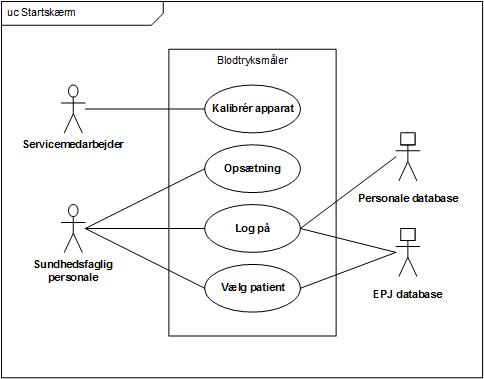
\includegraphics[width =0.7\textwidth , center]{billeder/UCStart}
\caption{\textbf{Use case diagram for startskærmen}}
\end{figure}
\begin{figure}[h!]
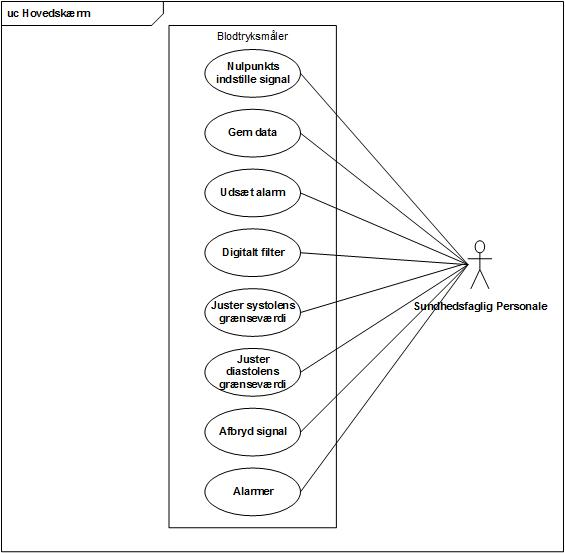
\includegraphics[width =0.7\textwidth , center]{billeder/UChoved}
\caption{\textbf{Use case diagram for hovedskærmen}}
\end{figure}
Af disse to Use case diagrammer ses de 13 Use cases der er for systemet. Det er her valgt at opdele disse Use cases i to Use case diagrammer, idet der haves to brugergrænseflader hhv.; startskærm og hovedskærm. Startskærmen fungerer som brugergrænsefladen, hvor det sundhedsfaglige personale kan logge på, hente patienten og dermed komme videre til hovedskærmen. Hovedskærmen fungerer som selve blodtryksmålersystemets brugerflade, det er herfra at det sundhedsfaglige personale kan igangsætte en måling, aflæse de ønskede værdier, stoppe en måling, afbryde evt. igangsatte alarmer og logge af igen, hvorefter startskærmen kommer frem igen. Det er disse brugergrænseflader som det sundhedsfaglige personale kan initiere med. \\
De 13 Use cases er: Kalibrér apparat, Opsætning, Log på, Vælg patient, Start måling, Nulpunkts juster signal, Slå digitalt filtet til/fra, Juster diastolens grænseværdi, Juster systolens grænseværdi, Alarmér, Udsæt alarm, Stop måling og Log ud. Hver enkel af disse Use cases beskrives detaljeret herunder i et fully-dressed Use case skema\\
\\
"Signalets vej" og opbygning beskrives\\\\



\newpage
\begin{table}[H]
\caption{Use case 1}\label{tab:tabel3}
\begin{tabular}{| l | >{\raggedright\arraybackslash}p{11cm} |}
   \hline
   \textbf{Use case 1} & \textbf{Kalibrér apparat}\\ \hline
   Mål: & Få kalibreret apparatet \\ \hline
   Initiering: & Startes af Servicemedarbejder\\ \hline
   Aktører:& Servicemedarbejder (primær)\\ \hline
   Referencer: & - \\ \hline
   Samtidige forekomster: & én kalibrering pr. apparat \\\hline
   Forudsætninger: & Blodtryksmålersystemet er tændt og tilsluttet kalibreringsudstyret.\\ \hline
   Resultat:& Apparatet er kalibreret\\ \hline
   Hovedscenarie:& 
1. Servicemedarbejder trykker på "Kalibrering"\newline
2. Systemet starter kalibreringen\newline
3. Besked: "Kalibreringen er fuldendt" vises på startskærmen\\\hline
Udvidelse/undtagelser: & - \\\hline
\end{tabular}
\end{table}

\begin{table}[H]
\caption{Use case 2}\label{tab:tabel3}
\begin{tabular}{| l | >{\raggedright\arraybackslash}p{11cm} |}
   \hline
   \textbf{Use case 2} & \textbf{Opsætning}\\ \hline
   Mål: & Få valgt port til NI-DAQ \\ \hline
   Initiering: & Startes af Sundhedsfaglig personale\\ \hline
   Aktører:& Sundhedsfaglig personale (primær) \\ \hline
   Referencer: &  -\\ \hline
   Samtidige forekomster: & Ét blodtryksmålersystem pr. opsætning \\\hline
   Forudsætninger: & Systemet tilsluttet en computer og tændt. \\ \hline
   Resultat:& Port valgt\\ \hline
   Hovedscenarie:& 
1. Sundhedsfaglig personale trykker på opsætnings dropdown på startskærmen\newline
2. Sundhedsfaglig personale vælger port \\\hline
Udvidelse/undtagelser: & -\\\hline
\end{tabular}
\end{table}



\begin{table}[H]
\caption{Use case 3}\label{tab:tabel3}
\begin{tabular}{| l | >{\raggedright\arraybackslash}p{11cm} |}
   \hline
   \textbf{Use case 3} & \textbf{Foretag måling}\\ \hline
   Mål: & Den valgte patients målinger foretages\\ \hline
   Initiering: & Startes af Sundhedsfaglig personale\\ \hline
   Aktører:& Sundhedsfaglig personale (primær), Personale database (sekundær), EPJ database(sekundær), Transducer (sekundær)\\ \hline
   Referencer: & Use case 2 \\ \hline
   Samtidige forekomster: & Én sundhedsfaglig person og én transducer pr. system \\\hline
   Forudsætninger: & Use case 2: Opsætning, er kørt succesfuldt\\ \hline
   Resultat:& Målingerne for den valgte patient er foretaget\\ \hline
   Hovedscenarie:& 
1. Sundhedsfaglig personale indtaster brugernavn og kode på startskærmen\newline
2. Sundhedsfaglig personale trykker på "Login"\newline
   \textit{$[$Undtagelse 1: Brugernavn og/eller kode indtastet forkert$]$}\newline
3. Besked: "Logget på" vises på startskærmen.  \newline
4. Sundhedsfaglig persoalen trykker på patient dropdown på startskærm \newline
5. Liste med patienter kommer frem\newline
6. Den ønskede patient vælges \newline
7. Nyt vindue kommer frem: Hovedskærmen\newline
8. Sundhedsfaglig personale trykker på "Tænd"\newline
9. Systemet indhenter data fra transduceren og starter timeren på hovedskærmen\newline
10. EKG, arterietryk og iltmætningskurve præsenteres kontinuert på hver sin graf. Puls, systole, diastole, middeltryk og iltmætning vises som talværdier på hovedskærmn. Data gemmes automatisk kontinuert i EPJ database. \newline
\textit{$[$Udvidelse 1: Slå digitalt filter til/fra$]$}\newline
\textit{$[$Udvidelse 2: Juster systolens/diastolens grænseværdi$]$}\newline
11. Sundhedsfaglig personale trykker på "Nulpunks justering"\newline
12. Systemet starter nulpunkts justeringen\newline
13. Besked "Nulpunkts justeringen er fuldent" vises på hovedskærmen
\\\hline
Udvidelse/undtagelser: & $[$Undtagelse 1: Brugernavn og/eller kode indtastet forkert$]$\newline
1.1 Besked: "Brugernavn og/eller kode indtastet forkert"\newline
1.2 Use case 3 starter forfra \newline\newline
$[$Udvidelse 1: Slå digitalt filter til/fra$]$\newline 
1.1 Sundhedsfaglig personale trykker på "Digitalt filter OFF" \newline
1.2 Systemet slår det digitale filter fra\newline
1.3 Sundhedsfaglig personale trykker på "Digitalt filter ON"\newline
1.4 Systemet slår det digitale filter til\newline\newline
$[$Udvidelse 2: Juster systolens/diastolens grænseværdi$]$\newline
2.1 Sundhedsfaglig personale trykker på "Systole op"/"Diastole op"\newline
2.2 Grænseværdien ændres 2.5mmHg op og intervallet vises på hovedskærmen\newline
2.3 Sundhedsfaglig personale trykker på "Systole ned"/"Diastole ned"\newline
2.4 Grænseværdien ændres 2.5mmHg ned og intervallet vises på hovedskærmen
\\\hline
\end{tabular}
\end{table}


\begin{table}[H]
\caption{Use case 4}\label{tab:tabel3}
\begin{tabular}{| l | >{\raggedright\arraybackslash}p{11cm} |}
   \hline
   \textbf{Use case 4} & \textbf{Alarmér}\\ \hline
   Mål: & Få startet alarmeringen ved overskridelse af grænseværdi \\ \hline
   Initiering: & Systemet starter denne Use case\\ \hline
   Aktører:& Sundhedsfaglig personale (sekundær)\\ \hline
   Referencer: & Use case 3 \\ \hline
   Samtidige forekomster: & - \\\hline
   Forudsætninger: & Målingen i Use case 3: Foretag måling, er kørt succesfuldt \\ \hline
   Resultat:& Alarmen starter\\ \hline
   Hovedscenarie:& 
1. Grænseværdi overskrides \newline
2. Alarm starter med lyd og tallet, hvis grænseværdi er overskredet, blinker.\newline
    \textit{$[$Udvidelse 1: Anden grænseværdi overskrides$]$} \newline
    \textit{$[$Udvidelse 2: Udsæt alarm$]$ }
\\\hline
Udvidelse/undtagelser: & $[$Udvidelse 1: Anden grænseværdi overskrides$]$ \newline
1.1. Endnu en grænseværdi overskrides\newline
1.2. Lyden fra første alarm fortsætter. Det nye tal som har overskredet grænseværdien blinker ligeledes.\newline
1.3 Use case afsluttet.\newline\newline
$[$Udvidelse 2: Udsæt alarm$]$\newline
2.1 Sundhedsfaglig person trykker på "Udsæt alarm"\newline
2.2 Systemet stopper alarmens lyd i et minut
\\\hline
\end{tabular}
\end{table}


\begin{table}[H]
\caption{Use case 5}\label{tab:tabel3}
\begin{tabular}{| l | >{\raggedright\arraybackslash}p{11cm} |}
   \hline
   \textbf{Use case 5} & \textbf{Stop måling}\\ \hline
   Mål: &  Få stoppet målingen og logget\\ \hline
   Initiering: & Startes af Sundhedsfaglig personale \\ \hline
   Aktører: & Sundhedsfaglig personale (primær) \\ \hline
   Referencer: & Use case 3\\ \hline
   Samtidige forekomster: & - \\\hline
   Forudsætninger: & Use case 3: Foretag måling, er kørt succesfuldt\\ \hline
   Resultat:& Signalet er stoppet, sundhedsfaglig personale er logget ud og vendt tilbage til startskærm.\\ \hline
   Hovedscenarie:& 
1. Sundhedsfaglig personale trykker på "Sluk"\newline
2. Målingen og timeren på hovedskærmen stopper.\newline 
3. Sundhedsfaglig personale trykker på "Log ud" \newline
4. Pop-up vindue kommer op: "Er du sikker?"\newline
5. Sundhedsfaglig personale trykker på "Ja"\newline
   \textit{$[$Udvidelse 1: Tryk på "Nej"$]$}\newline
6. Startkærmen kommer frem og ny måling kan foretages\\\hline
Udvidelse/undtagelser: & $[$Udvidelse 1: Tryk på "Nej"$]$\newline
1.1 Sundhedsfaglig personale trykker "Nej"\newline
1.2 Kommer tilbage til hovedskærmen\newline
1.3 Use case afsluttet\\\hline
Udvidelse/undtagelser: & -\\\hline
\end{tabular}
\end{table}




\newpage 
\newpage 
\newpage
\newpage



\section{Ikke-funktionelle krav}
De ikke-funktionelle krav er opsat efter FURPS+ metoden. De er prioriteret efter MoSCoW metoden:
\begin{itemize}
\item \textbf{M}ust (skal være med)
\item \textbf{S}hould (bør være med, hvis muligt)
\item \textbf{C}ould (kunne have med, hvis det ikke går i vejen for noget andet)
\item \textbf{W}on't/\textbf{W}ould (tager det ikke med nu, men kan komme med i fremtidige opdateringer)
\end{itemize}

\subsection{FURPS+ med MoSCoW}
\begin{enumerate}
\item \textbf{Functionality}
\begin{enumerate}
\item (\textbf{M}) Programmet skal have et digitalt filter til udglatning af blodtrykssignal
\item (\textbf{M})Programmet skal give alarm når grænseværdier overskrides med lyd og hvor den overskredede grænseværdi blinker på skærmen.
\item (\textbf{M}) Programmet skal kunne gemme blodtrykssignalet i en database.
\end{enumerate}
\item \textbf{Usability}
\begin{enumerate}
\item (\textbf{S}) Programmet skal have to window forms: startskærm, der fungerer som  EPJ systemet og hovedskærm, hvilken fungerer som selve blodtryksmålerens grænseflade.
\item (\textbf{M}) Programmet skal have en "Login" knap på startskærmen
\item (\textbf{M}) Programmet skal have en "Kalibrering" knap på startskærmen
\item (\textbf{M}) Sundhedsfagligt personale skal kunne ændre "devicename/enhedsnavn" i dropdown på startskærmen
\item (\textbf{S}) Programmet skal indeholde en dropdown, hvor patienten kan vælges, på startskærmen
\item (\textbf{M}) Programmet skal have en "Nulpunkts indstilling" knap på hovedskærmen
\item (\textbf{M}) Programmet skal have en knap til at slå det digitale filter fra og til på hovedskærmen
\item (\textbf{M}) Programmet skal have knapper til at justere systolisk og diastolisk grænseværdi-intervaller op og ned, på hovedskærmen
\item (\textbf{M}) Programmet skal have en "Udsæt alarm" knap på hovedskærmen
\item (\textbf{M}) Programmet skal have en "Tænd" knap på hovedskærmen.
\item (\textbf{M}) Programmet skal have en "Sluk" knap på hovedskærmen
\item (\textbf{M}) Programmet skal have en "Afbryd" knap på hovedskærmen.
\item (\textbf{M}) Teksten på startskærmen skal kunne læses fra 2 meters afstand ved synsstyrke i intervallet på +/-1
\item (\textbf{M}) Teksten og graferne på hovedskærmen skal kunne læses fra 2 meters afstand ved synsstyrke i intervallet på +/-1 
\item (\textbf{M}) Programmet skal præsentere data på grafer på følgende måde (Se afsnit nedenfor)
\begin{itemize}
\item EKG vises i lysegrøn
\item Arterietryk vises i rød
\item Iltmætning/saturation i lyseblå
\end{itemize}
\item (\textbf{M}) Programmet skal præsentere data i tal på følgende måde (Se afsnit nedenfor)
\begin{itemize}
\item Hjertefrekvens i lysegrøn
\ Systolisk samt diastolisk tryk i rødt, ligeledes middelblodtrykket i parentes under i rødt.
\end{itemize}
\begin{figure}[h!]
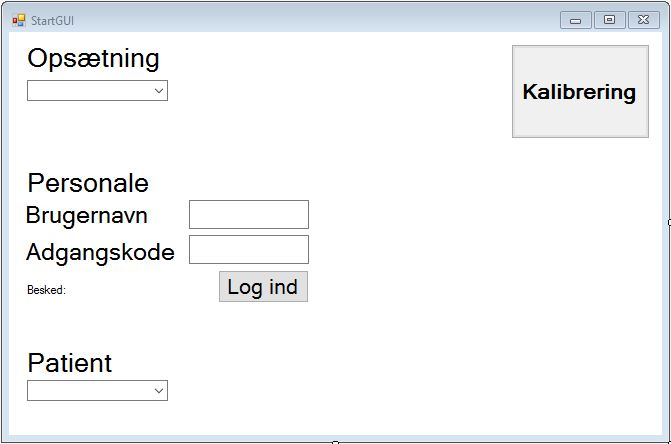
\includegraphics[width =0.4\textwidth , center]{billeder/skitseStart}
\caption{Skitse af startskærmen, hvilken repræsenterer EPJ systemet}
\end{figure}
\begin{figure}[h!]
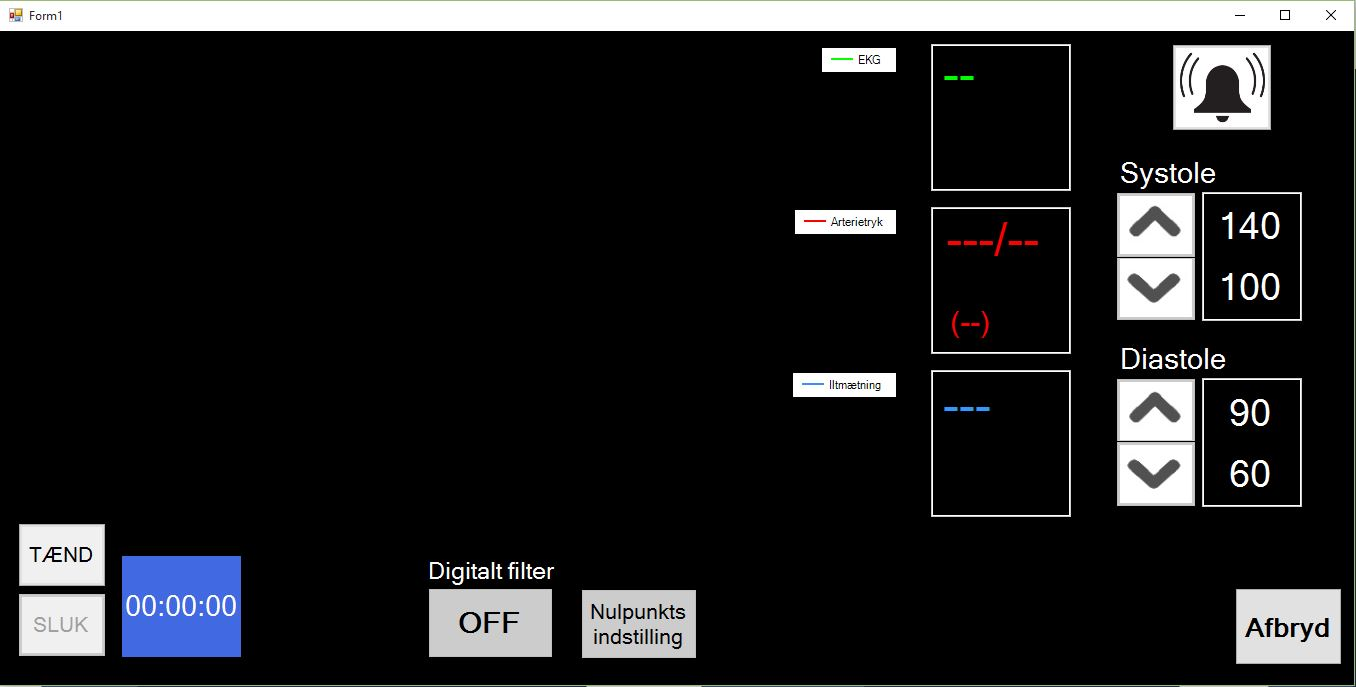
\includegraphics[width =1.0\textwidth , center]{billeder/skitseHoved}
\caption{Skitse af hovedskærmen, hvilken repræsenterer en blodtryksmålers brugerflade}
\end{figure}
\end{enumerate}
\item \textbf{Reliability}
\begin{enumerate}
\item (\textbf{S}) INGEN RELIABILITY KRAV ENDNU
\end{enumerate}
\item \textbf{Performance}
\begin{enumerate}
\item (\textbf{S}) Tiden der går før måling af data påbegynder / vises i grafer må maksimalt være 2 sek.
\item (\textbf{M}) Tiden der går fra at data, herunder puls, diastolisk tryk, systolisk tryk, middeltryk og iltmætning, er analyseret til at data'en er gemt i EPJ database må være 2 sek. med en tolerance på +/-15\%  
\end{enumerate}
\item \textbf{Supportability}
\begin{enumerate}
\item (\textbf{M}) Softwaren skal være opbygget efter trelagsmodellen (Data-View-Model)
\end{enumerate}
\item \textbf{+ Test conditions}
\begin{enumerate}
\item (\textbf{M}) Der skal være adgang til en computer med Windows 7, 8 eller 10 - computeren skal minimum have 4 GB RAM.
\item (\textbf{M}) Der skal være adgang til en computer hvor National Instruments er installeret.
\end{enumerate}
\end{enumerate}
\chapter{Arkitektur}
\section{Hardware design}
\subsection{Implementering}
\subsection{Modultest}
\section{Software design}
\subsection{Implementering}
\subsection{Unittest}
\section{Integrationstest}
\chapter{Accepttest}
\section{Indledning}
Accepttestene skal vise om kravene der er opstillet for blodtryksmålersystmet lever op til de standarder der er sat op for at produktet aktivt kan indgå i en hverdag på afdelingen.\\
Accepttestene er er opfølgning af kravsspecifikationen, hvilket sikre at alle krav er overholdt og dermed opnået.\\\\
Kort beskrivelse hvordan data indhentes\\\\
Når der i feltet Godkendt er et flueben, betyder det at testen er godkendt. Hvis der er et flueben i parenteser, betyder det at den er delvis godkendt. \\

\section{Accepttest for funktionelle krav}
\subsection{Opstilling}
Billede indsættes - haves ikke endnu

\begin{table}[H]
\caption{Accepttest for Use case 1}\label{tab:tabel8}
\begin{tabular}{|>{\raggedright\arraybackslash}p{2.5cm}| >{\raggedright\arraybackslash}p{2.9cm} | >{\raggedright\arraybackslash}p{2.9cm} | >{\raggedright\arraybackslash}p{2.9cm} | >{\raggedright\arraybackslash}p{2.8cm} |}
   \hline
   \textbf{Use case 1: Kalibrer apparat} &\textbf{Test}& \textbf{Prækondition} & \textbf{Forventet resultat} & \textbf{Godkendt/ kommentar}\\ \hline
   Normalforløb:& Tryk på "Kalibrering" & Blodtryksmåleren er tændt og tilsluttet kalibreringsudstyret. & Systemet er kalibreret og besked "Kalibreringen er fuldendt" vises på startskærmen & IKKE TESTBAR\\\hline
\end{tabular}
\end{table}

\begin{table}[H]
\caption{Accepttest for Use case 2}\label{tab:tabel8}
\begin{tabular}{|>{\raggedright\arraybackslash}p{2.5cm}| >{\raggedright\arraybackslash}p{2.9cm} | >{\raggedright\arraybackslash}p{2.9cm} | >{\raggedright\arraybackslash}p{2.9cm} | >{\raggedright\arraybackslash}p{2.8cm} |}
   \hline
   \textbf{Use case 2: Opsætning} &\textbf{Test}& \textbf{Prækondition} & \textbf{Forventet resultat} & \textbf{Godkendt/ kommentar}\\ \hline
   Normalforløb:& Tryk på opsætningens dropdown  & Systemet er tilsluttet en computer og er tændt & Liste med porte kommer frem. & \\\hline
   &Port vælges & Systemet er tilsluttet en computer og er tændt & Port valgt &\\\hline
\end{tabular}
\end{table}

\begin{table}[H]
\caption{Accepttest for Use case 3}\label{tab:tabel8}
\begin{tabular}{|>{\raggedright\arraybackslash}p{2.5cm}| >{\raggedright\arraybackslash}p{2.9cm} | >{\raggedright\arraybackslash}p{2.9cm} | >{\raggedright\arraybackslash}p{2.9cm} | >{\raggedright\arraybackslash}p{2.8cm} |}
   \hline
   \textbf{Use case 3: Log på} &\textbf{Test}& \textbf{Prækondition} & \textbf{Forventet resultat} & \textbf{Godkendt/ kommentar}\\ \hline
   Normalforløb:& Indtast brugernavn "abcd" og kode "1234" & Port valgt & Korrekt indtastning fuldendt & \\\hline
   &Tryk "Login" & Port valgt & Besked: "Logget på" og den sundhedsfaglige er dermed logget på &\\\hline
\end{tabular}
\end{table}



\begin{table}[H]
\caption{Accepttest for Use case 3}\label{tab:tabel8}
\begin{tabular}{|>{\raggedright\arraybackslash}p{2.5cm}| >{\raggedright\arraybackslash}p{2.9cm} | >{\raggedright\arraybackslash}p{2.9cm} | >{\raggedright\arraybackslash}p{2.9cm} | >{\raggedright\arraybackslash}p{2.8cm} |}
   \hline
   \textbf{Use case 3: Log på} &\textbf{Test}& \textbf{Prækondition} & \textbf{Forventet resultat} & \textbf{Godkendt/ kommentar}\\ \hline
   Undtagelse 1: Brugernavn og/eller kode indtastet forkert & Indtast brugernavn "efgh" og kode "1234"& Port valgt & Forkert kombinition indtastet &  \\\hline
   &Tryk "Login" & Port valgt & Besked: "Brugernavn og/eller kode indtastet forkert" &\\\hline
\end{tabular}
\end{table}






\begin{table}[H]
\caption{Accepttest for Use case 4}\label{tab:tabel8}
\begin{tabular}{|>{\raggedright\arraybackslash}p{2.5cm}| >{\raggedright\arraybackslash}p{2.9cm} | >{\raggedright\arraybackslash}p{2.9cm} | >{\raggedright\arraybackslash}p{2.9cm} | >{\raggedright\arraybackslash}p{2.8cm} |}
   \hline
   \textbf{Use case 4: Vælg patient} &\textbf{Test}& \textbf{Prækondition} & \textbf{Forventet resultat} & \textbf{Godkendt/ kommentar}\\ \hline
   Normalforløb:& Tryk på patient dropdown på startskærm & En sundhedsfaglig er logget på & Liste med patienter kommer frem  & \\\hline
   & Marker patienten "Peter Petersen" og dobbeltklik på denne & Den sundhedsfaglige er logget på & Nyt vindue kommer frem: Hovedskærmen &\\\hline
\end{tabular}
\end{table}


\begin{table}[H]
\caption{Accepttest for Use case 5}\label{tab:tabel8}
\begin{tabular}{|>{\raggedright\arraybackslash}p{2.5cm}| >{\raggedright\arraybackslash}p{2.9cm} | >{\raggedright\arraybackslash}p{2.9cm} | >{\raggedright\arraybackslash}p{2.9cm} | >{\raggedright\arraybackslash}p{2.8cm} |}
   \hline
   \textbf{Use case 5: Start signal} &\textbf{Test}& \textbf{Prækondition} & \textbf{Forventet resultat} & \textbf{Godkendt/ kommentar}\\ \hline
   Normalforløb:& Tryk på "Tænd"& Patient valgt og transduceren er tilsluttet & Systemet indhenter data og starter timer. EKG, arterietryk og iltmætningskurve præsenteres kontinuert på hver sin graf. Puls, systole, diastole, middeltryk og iltmætning vises som talværdier på hovedskærmen. Data gemmes automatisk kontinuert i EPJ database & \\\hline
\end{tabular}
\end{table}

\begin{table}[H]
\caption{Accepttest for Use case 6}\label{tab:tabel8}
\begin{tabular}{|>{\raggedright\arraybackslash}p{2.5cm}| >{\raggedright\arraybackslash}p{2.9cm} | >{\raggedright\arraybackslash}p{2.9cm} | >{\raggedright\arraybackslash}p{2.9cm} | >{\raggedright\arraybackslash}p{2.8cm} |}
   \hline
   \textbf{Use case 6: Nulpunkts juster signal } &\textbf{Test}& \textbf{Prækondition} & \textbf{Forventet resultat} & \textbf{Godkendt/ kommentar}\\ \hline
   Normalforløb:& Tryk på "Nulpunkts justering" & Signalet er startet og kører & Systemet starter nulpunkts justeringen. Besked " Nulpunkts justering er fuldendt" vises på hovedskærmen &\\\hline
\end{tabular}
\end{table}



\begin{table}[H]
\caption{Accepttest for Use case 7}\label{tab:tabel8}
\begin{tabular}{|>{\raggedright\arraybackslash}p{2.5cm}| >{\raggedright\arraybackslash}p{2.9cm} | >{\raggedright\arraybackslash}p{2.9cm} | >{\raggedright\arraybackslash}p{2.9cm} | >{\raggedright\arraybackslash}p{2.8cm} |}
   \hline
   \textbf{Use case 7: Slå digitalt filter til/fra} &\textbf{Test}& \textbf{Prækondition} & \textbf{Forventet resultat} & \textbf{Godkendt/ kommentar}\\ \hline
   Normalforløb:& Tryk på "Digitalt filter OFF" & Signalet er startet & Systemet slår det digitale filter fra. Grafen ses at være ufiltreret(råt) og knappen ændrer navn. &\\\hline
   &Tryk på "Digitalt filter ON" & Signalet er startet & Systemet slår det digitale filter til. Grafen ses at være filtreret og knappen ændrer navn. &\\\hline
\end{tabular}
\end{table}


\begin{table}[H]
\caption{Accepttest for Use case 8}\label{tab:tabel8}
\begin{tabular}{|>{\raggedright\arraybackslash}p{2.5cm}| >{\raggedright\arraybackslash}p{2.9cm} | >{\raggedright\arraybackslash}p{2.9cm} | >{\raggedright\arraybackslash}p{2.9cm} | >{\raggedright\arraybackslash}p{2.8cm} |}
   \hline
   \textbf{Use case 8: Juster systolens grænseværdi } &\textbf{Test}& \textbf{Prækondition} & \textbf{Forventet resultat} & \textbf{Godkendt/ kommentar}\\ \hline
   Normalforløb:& Tryk på "Systole op"& Signalet er startet & Grænseværdien ændres 2.5 mmHg op og intervallet vises på hovedskærmen &\\\hline
   &Tryk på "Systole ned" & Signalet er startet & Grænseværdien ændres 2.5 mmHg ned og intervallet vises på hovedskærmen & \\\hline
\end{tabular}
\end{table}

\begin{table}[H]
\caption{Accepttest for Use case 9}\label{tab:tabel8}
\begin{tabular}{|>{\raggedright\arraybackslash}p{2.5cm}| >{\raggedright\arraybackslash}p{2.9cm} | >{\raggedright\arraybackslash}p{2.9cm} | >{\raggedright\arraybackslash}p{2.9cm} | >{\raggedright\arraybackslash}p{2.8cm} |}
   \hline
   \textbf{Use case 9: Juster diastolens grænseværdi } &\textbf{Test}& \textbf{Prækondition} & \textbf{Forventet resultat} & \textbf{Godkendt/ kommentar}\\ \hline
   Normalforløb:& Tryk på "Diastole op"& Signalet er startet & Grænseværdien ændres 2.5 mmHg op og intervallet vises på hovedskærmen &\\\hline
   &Tryk på "Diastole ned" & Signalet er startet & Grænseværdien ændres 2.5 mmHg ned og intervallet vises på hovedskærmen & \\\hline
\end{tabular}
\end{table}

\begin{table}[H]
\caption{Accepttest for Use case 10}\label{tab:tabel8}
\begin{tabular}{|>{\raggedright\arraybackslash}p{2.5cm}| >{\raggedright\arraybackslash}p{2.9cm} | >{\raggedright\arraybackslash}p{2.9cm} | >{\raggedright\arraybackslash}p{2.9cm} | >{\raggedright\arraybackslash}p{2.8cm} |}
   \hline
   \textbf{Use case 10: Alarmér } &\textbf{Test}& \textbf{Prækondition} & \textbf{Forventet resultat} & \textbf{Godkendt/ kommentar}\\ \hline
   Normalforløb:& Grænseværdi overskrides& Signalet er startet & Alarm starter med lyd og tallet, hvis grænseværdi er overskredet, blinker &\\\hline
\end{tabular}
\end{table}



\begin{table}[H]
\caption{Accepttest for Use case 10}\label{tab:tabel8}
\begin{tabular}{|>{\raggedright\arraybackslash}p{2.5cm}| >{\raggedright\arraybackslash}p{2.9cm} | >{\raggedright\arraybackslash}p{2.9cm} | >{\raggedright\arraybackslash}p{2.9cm} | >{\raggedright\arraybackslash}p{2.8cm} |}
   \hline
   \textbf{Use case 10: Alarmér } &\textbf{Test}& \textbf{Prækondition} & \textbf{Forventet resultat} & \textbf{Godkendt/ kommentar}\\ \hline
   Udvidelse 1: Anden grænseværdi overskrides & Endnu en grænseværdi overskrides & Signalet er er startet og en alarm er startet & Lyd fra første alarm fortsætter og det nye tallet som har overskredet grænseværdien blinker ligeledes &\\\hline
\end{tabular}
\end{table}



\begin{table}[H]
\caption{Accepttest for Use case 11}\label{tab:tabel8}
\begin{tabular}{|>{\raggedright\arraybackslash}p{2.5cm}| >{\raggedright\arraybackslash}p{2.9cm} | >{\raggedright\arraybackslash}p{2.9cm} | >{\raggedright\arraybackslash}p{2.9cm} | >{\raggedright\arraybackslash}p{2.8cm} |}
   \hline
   \textbf{Use case 11: Udsæt alarm } &\textbf{Test}& \textbf{Prækondition} & \textbf{Forventet resultat} & \textbf{Godkendt/ kommentar}\\ \hline
   Normalforløb:& Tryk på "Udsæt alarm" & Alarmering er startet & Systemet stopper alarmens lyd i et minut &\\\hline
\end{tabular}
\end{table}


\begin{table}[H]
\caption{Accepttest for Use case 12}\label{tab:tabel8}
\begin{tabular}{|>{\raggedright\arraybackslash}p{2.5cm}| >{\raggedright\arraybackslash}p{2.9cm} | >{\raggedright\arraybackslash}p{2.9cm} | >{\raggedright\arraybackslash}p{2.9cm} | >{\raggedright\arraybackslash}p{2.8cm} |}
   \hline
   \textbf{Use case 12: Stop måling } &\textbf{Test}& \textbf{Prækondition} & \textbf{Forventet resultat} & \textbf{Godkendt/ kommentar}\\ \hline
   Normalforløb:& Tryk på "Sluk" & Signalet er startet & Målingen, signalet og timer stopper &\\\hline
\end{tabular}
\end{table}

\begin{table}[H]
\caption{Accepttest for Use case 13}\label{tab:tabel8}
\begin{tabular}{|>{\raggedright\arraybackslash}p{2.5cm}| >{\raggedright\arraybackslash}p{2.9cm} | >{\raggedright\arraybackslash}p{2.9cm} | >{\raggedright\arraybackslash}p{2.9cm} | >{\raggedright\arraybackslash}p{2.8cm} |}
   \hline
   \textbf{Use case 13: Log ud } &\textbf{Test}& \textbf{Prækondition} & \textbf{Forventet resultat} & \textbf{Godkendt/ kommentar}\\ \hline
   Normalforløb:& Tryk "Log ud" & Signalet er stoppet & Pop-up vindue kommer op: "Er du sikker?" &\\\hline
   &Tryk "Ja"&Signalet og målingen er stoppet& Startskærmen kommer frem og ny måling kan foretages &\\\hline
\end{tabular}
\end{table}


\begin{table}[H]
\caption{Accepttest for Use case 13}\label{tab:tabel8}
\begin{tabular}{|>{\raggedright\arraybackslash}p{2.5cm}| >{\raggedright\arraybackslash}p{2.9cm} | >{\raggedright\arraybackslash}p{2.9cm} | >{\raggedright\arraybackslash}p{2.9cm} | >{\raggedright\arraybackslash}p{2.8cm} |}
   \hline
   \textbf{Use case 13: Log ud } &\textbf{Test}& \textbf{Prækondition} & \textbf{Forventet resultat} & \textbf{Godkendt/ kommentar}\\ \hline
Udvidelse 1: Tryk på "Nej" &Tryk "Nej" & Signalet og målingen er stoppet & Kommer tilbage til hovedskærmen &\\\hline
\end{tabular}
\end{table}



\newpage

\newpage

\newpage

\section{Accepttest for ikke-funktionelle krav}

\begin{longtable}{|>{\raggedright\arraybackslash}p{1.1cm}| >{\raggedright\arraybackslash}p{2.7cm} | >{\raggedright\arraybackslash}p{2.7cm} | >{\raggedright\arraybackslash}p{2.7cm} | >{\raggedright\arraybackslash}p{2.2cm} |>{\raggedright\arraybackslash}p{2.2cm}|}
   \caption{Accepttest for ikke-funktionelle krav}\label{tab:label13}
\\ \hline   
\textbf{Krav nr.}&\textbf{Krav} &\textbf{Test}& \textbf{Forventet resultat} & \textbf{Resultat} & \textbf{Godkendt/ kommentar}\\ \hline
  1.1 & Programmet skal have et digitalt filter til udglatning af blodtrykssignal & Tænd det digitale filter og tjek udglatningen & Signalet bliver mindre "råt"(udglattet) & & \\\hline
  1.2 & Programmet skal give alarm når grænseværdier overskrides med lyd og hvor den overskredede grænse værdi blinker på skærmen. & Overskrid en grænseværdi og tjek alarmering & Alarmen starter& & \\\hline
  1.3 & Programmet skal kunne gemme blodtrykssignalet i en database & Indsend signal og gå ind i databasen og se værdier & Der ligger værdier i databasen & & \\\hline\hline
  2.1 & Programmet skal have to window form: startskærm,der fungerer som EPJ systemet, og hovedskærm, hvilken fungerer som selve blodtryksmåleren & Start program og tjek dette & Der er to window forms & & \\\hline
  2.2 & Programmet skal have en "Login" knap på startskærmen & Start program og tjek startskærm & Startskærmen har en "Login" knap & & \\\hline
  2.3 & Programmet skal have en "Kalibrering" knap på startskærmen & Start program og tjek startskærm & Startskærmen har en "Kalibrering" knap & & \\\hline
  2.4 &Sundhedsfaglig personale skal kunne ændre "device/enhedsnavn" i dropdown på startskærm & Start program og tjek startskærm & Der er en opsætnings dropdown på startskærmen & & \\\hline
  2.5 & Programmet skal indeholde en dropdown, hvor patienten kan vælges på startskærmen & Start program og tjek startskærm & Startskærmen har en dropdown med patienter & & \\\hline
  2.6 & Programmet skal have en "Nulpunkts indstilling" knap på hovedskærmen & Start program og tjek hovedskærm & Der er en "Nulpunkts indstilling" knap på hovedskærmen & & \\\hline
  2.7 & Programmet skal have en knap, til at slå det digitale filter fra og til, på hovedskærmen & Start program og tjek hovedskærm & Der er en "Digital filter" knap på hovedskærmen & & \\\hline
  2.8 & Programmet skal have knapper, til at justere systolisk og diastolisk grænseværdiintervaller op og ned, på hovedskærmen & Start program og tjek hovedskærm & Der er ialt fire knapper, som justerer grænseværdierne på hovedskærmen & & \\\hline
  2.9 & Programmet skal have en "Udsæt alarm" knap på hovedskærmen & Start program og tjek hovedskærm & Der er en "Udsæt alarm" på hovedskærmen & & \\\hline
  2.10 & Programmet skal have en "Tænd" knap på hovedskærmen & Start program og tjek hovedskærm & Hovedskærmen har en "Tænd" kanp& & \\\hline
  2.11 & Programmet skal have en "Sluk" knap på hovedskærmen & Tjek hovedskærm & Hovedskærmen har en "Sluk" knap & & \\\hline
  2.12 & Programmet skal have en "Afbryd" knap på hovedskærmen & Start program og tjek hovedskærm & Der er en "Afbryd" knap på hovedskærmen & & \\\hline
  2.13 & Teksten på startskærmen skal kunne aflæs fra 1 meters afstand med en synsstyrke i intervallet +/-1 & 10 personer med synsstyrke i intervallet +/-1 skal teste startskærmen  & Alle 10 personer kan læse teksten tydeligt & & \\\hline
  2.14 & Teksten og graferne på hovedskærmen skal kunne læses fra 2 meters afstand ved synsstyrke i intervellet på +/-1 & 10 personer med synsstyrke i intervallet +/-1 skal teste hovedskærmen & Alle 10 personer kan læse grafer og teksten på hovedskærmen & & \\\hline
  2.15 & Programmet skal præsentere grafer efter standard & Start program og tjek farver & farverne på grafen er efter standard & & \\\hline
  2.16 & Programmet skal præsentere data i tal efter standard & Start program og tjek at talværdiernes farve er efter standard & Talværdiernes farve er efter standard & & \\\hline\hline
  3.1 & Ingen krav endnu & & & & \\\hline\hline
  4.1 & Tiden der går før målingen af data påbegynder/vises i grafer må maksimalt være 2.0 sek. & Stopur igangsættes samtidig med at signalet tændes & Stopuret viser 2 sek. eller mindre & & \\\hline
  4.2 & Tiden der går fra at data er analyseret til at data er gemt i database må være 2.0 sek. med en tolerance på +/- 15\% & - & & & \\\hline\hline
  5.1 & Softwaren skal være opbygget efter trelagsmodellen & Se programopbygningen & Softwaren er opbygget efter trelagsmodellen & & \\\hline\hline
  6.1 & Der skal være adgang til en computer med Windows 7, 8 eller 10 - computeren skal minimum have 4 GB RAM & & & & \\\hline
  6.2 & Der skal være adgang til en computer hvor National Instruments er installeret & & & & \\\hline
\end{longtable}

\section{Godkendelses formular}
\begin{table}[h!]
\label{tab:tabel14}
\begin{tabular}{| l | >{\raggedright\arraybackslash}p{12cm} |}
   \hline
   \textbf{Dato for test} &\\ \hline
   \textbf{Godkendes af:} & \\ \hline
\end{tabular}
\end{table}
\textbf{Ved underskrivelse af dette dokument godkendes den kørte accepttest}
\newline
\textbf{Sted og dato:}\\
\\
\\
\begin{table}
[h!]
\begin{tabular}{ l lllllllll l}
--------------------------------------&&&&&&&&&&--------------------------------------\\ 
Kundens underskrift &&&&&&&&&&Leverandørens underskrift\\
\end{tabular}
\end{table}
